\documentclass[12pt]{article}
\usepackage{xeCJK}%preamble part
\usepackage{graphicx}
\usepackage{indentfirst}
\usepackage[a4paper, inner=1.5cm, outer=3cm, top=2cm, bottom=3cm, bindingoffset=1cm]{geometry}
\usepackage{epstopdf}
\usepackage{array}
\usepackage{fontspec}
\usepackage{gensymb}
\usepackage[citecolor=blue]{hyperref}
\usepackage{amsmath}
\usepackage{makecell}
\usepackage[lofdepth,lotdepth]{subfig}
\DeclareMathOperator*{\argmax}{argmax}
\setCJKmainfont[BoldFont={SimHei}]{SimSun}
\setCJKmonofont{SimSun}
\setmainfont{Times New Roman}
\newCJKfontfamily[hei]\heiti{SimHei}
\setlength{\extrarowheight}{4pt}
\setlength{\parindent}{1cm}
\begin{document}
\title{\textbf{\fontsize{15.75pt}{\baselineskip}{用户型德语初学者词典Klick Auf Deutsch Hilfer设计理念}}}
\author{\fontsize{12pt}{\baselineskip}{计41 牛行知 数33 赵丰}}

\maketitle
\renewcommand{\abstractname}{摘要}
\renewcommand*\contentsname{目录}
\begin{abstract}
在国内外语学习的热潮下双语词典的编纂一直是为人们所忽视的主题,传统词典一直由少数专家把关,编一部词典的周期长,门槛高;现代信息技术的进步为使用计算机网络技术进行协作式编辑,充分考虑用户需求,缩短编辑周期和提高实用性方面提供了可能。本次项目试图以用户型德语初学者词典为突破口探索这种可能性。目前已经实现了词典的浏览和在线编辑模块。
\end{abstract}
\tableofcontents
\large
\twocolumn
\setlength{\columnseprule}{1pt}

\section[问题背景]{问题背景:我国双语学习型词典的设计缺位}
尽管英汉词典学是我国外语人才培养的一个二级学科,但我国真正流行的词典几乎都是所引进或合作编纂出版的外来词典,其编纂设计者与使用者形成了主客二分的疏离关系,设计者对于需求的认知主要源于编者主体的专业知识判断,而非对实际用户需求调研的结果。\cite{Bib1}

我国原创英汉汉英类词典,在国内词典市场的份额缺失严重,这和脱离用户需求,盲目照翻单语词典不无关系。

从表面上看,我国电子词典呈现出一片繁荣景象,所涉语言从英汉延伸至其他小语种,但实际情况是电子产品公司与计算机软件开发公司对电子词典表现出极大的热情,辞书出版机构将纸制词典的电子版权转让给电子出版商,而后者只是简单地把印在纸上的东西搬进芯片。

欧美电子词典以辞书为本体来开发电子词典,注重词典数据库的建设,而我国内地则是以电子为本体,先是由IT公司开发,出现问题后又转向引进权威词典。\cite{Bib2}

\section{设计目标描述}
	电子词典的核心功能是单词查询的浏览功能。
	电子词典的界面设计一方面要继承纸制词典的风格,另一方面在不同的媒介下有一定的发挥空间。
	
	为实现上述设计目标,我们以网页为平台开发了Klick Auf Deutsch Hilfer。
	在开发过程中,为了提高编辑工作效率,我们设计了用户编辑模块。
\section{单词查询}

\subsection{\textbf{\fontsize{12pt}{\baselineskip}{数据视角}}}
	我们设计词典抛弃了一般电子词典采用的急键值加表项的方式,而采用超文本标记语言xml组织每一个词项。单独的xml文件以词条的编号命名,如1.xml表示名词类中的第一个,词项是Abend;V100.xml表示动词类中的第100个,词项是wissen.
	
	xml可以自定义元素和属性,为此我们采用了文档类型定义dtd的方法,考虑到不同词性的词有不同的属性,每一个词性我们单独定义了一个dtd文件,在xml文档的头部,显示指明了它被哪一个dtd所约束,如NounModel.dtd。虽然不同词性的词有不同的dtd,但其大致结构相同。具体说来,每一个合法的xml首先都要有一个根元素名为Entry.Entry下必须依次出现元素Stichwort,Einheit/Anteil,zusammengesetzteWörter,
Synonymegruppe,Antonymegruppe,
Kollokationen,AllgemeineErläuterungen.

这里有的子元素结构比较简单,比如Stichwort下只包含了词形的信息。
Einheit/Anteil元素是适配考虑到清华大学德语教学正在使用的教材为每个单词提供的其所在单元和所在单元具体模块的信息。
zusammengesetzteWörter元素提供德语中的和该词有关的复合词的信息,
由于德语中复合词数量更多,相应的我们在zusammengesetzteWörter
下设了KompositaCollection和abgeleiteteWörter两个子元素,
分别包含合成词类和派生词类。在合成词类下,为支持后期多种检索方式,我们将其主要分为K\_和 \_K型,分别表示这个词项在该合成词的位置
是在前面还是后面,派生词类下对每个由该词项派生的词必须注明它的词性,否则按照dtd的语法检查规则,整篇文档就是不合法的。

对于Entry下接下来的三个元素,分别表示同义词集合、反义词集合和词组集合,其中我们在编辑的过程中发现,同反义词集合具有稀疏性。

整个词条中最重要的部分是AllgemeineErläuterungen,其结构也最复杂。考虑到一词多义的可能性,该“一般性释义”下设若干个Eintrag,
至少要有一个Eintrag.每一个Eintrag有Chinesisch和BeispielSammlung
两个子元素,分别是汉语释义和例句集,每一个例句集是由若干个
Beispiel组成的,而每一个Beipiel由Satz和Übersetzung组成。该部分对
整个文档树的深度贡献最大。

同时,我们考虑到单词之间错综复杂的语义关系,在Eintrag的相关子元素下设置了link属性,其值为相对应单词的文件名称,如essen词项下<\_K link=''1.xml''>Abendessen<\/K>就表示Abendessen可以链接到Abend.这种方法不仅为展示数据提供了统一个接口,还为用网络的方法做关联分析提供了数据基础。
\subsection{\textbf{\fontsize{12pt}{\baselineskip}{界面视角}}}
\section{用户编辑}

\section{背单词}
我们打算基于已有的词典内容开发背单词的模块,传统的背单词往往基于简单的随机因子和分数累加,在开发之前,我们仔细学习了Item Response
Theory,并以此理论为基础,建立单词测试的数学模型,用统计学中分析数据的方法,在数据库和CS架构的技术基础上尝试实现背单词模块,目前该
模块正在开发过程中。
\subsection{\textbf{\fontsize{12pt}{\baselineskip}{词汇量统计方法}}}
\cite{Bib4}中给出了估计正常人遇到的词汇量的基本方法,首先统计出Alphabetical Type(N)与语料库规模(M)的关系,Herdan's Law指出N是M的幂函数且幂指数小于1,其次通过抽样调查的方法统计某一特定人群在一段时间内exposed to 语言输入的tokens,对这些tokens进行统计去重再外推即得到encountered AT值。
传统的词汇测量方法是基于Classical Test Theory对于每个test item,一般结果是二值的,即只有对和错两个result,累加后的结果可以作为observed score。CTT认为X=T+E,T是true score,E是error.
CTT还有三个基本假设:
\begin{enumerate}
\item{E的期望为0}
\item{T和E不相关}
\item{不同次测量结果(对不同participants)相互独立}
\end{enumerate}
该测量的性能评估用reliability表示,其数学定义为
\begin{equation}
\rho_{XT}^2=\frac{\sigma_T^2}{\sigma_X^2}
\end{equation}
在心理学领域,要测量某个latent variable,不能采用独立重复试验的方法,如果要基于单次测量估计$\rho_{XT}$,该单次测量应该在subscale上应该由同样能反应出被测量laten variable 水平的item组成。
基于不同participants,可以得到item 矩阵,分析该item矩阵可估计$\rho_{XT}$。该方法的数学模型如下:
假设一test有k个items $u_j,j=1,..,k$,对第i个participant其总得分为:
\begin{equation}
X_i=\sum_{j=1}^k U_{ij}
\end{equation}
上式中$U_{ij}$表示对第i个参与者在第j个item上observed score。
可以证明,Cronbach's alpha是$\rho_{XT}$的下界。
\begin{equation}
\alpha=\frac{k}{k-1}(1-\frac{\sum_{i=1}^k \sigma_{U_j}^2}{\sigma_X^2})
\end{equation}
$\alpha$介于0,1之间,用于评估Test性能,一般认为$\alpha$值在0.9以上会有redundacy of items,但对于individual high-stakes testing这又是必要的。
在CTT框架下,$\alpha$只能用于评估Test总体性能,如果要做item analysis,对于每个item,计算p value(表征item difficulty)和item-total correlation(表征 discrimination).
CTT的问题在于评估Test性能和被试者特征(examinee characteristics)有关,而且对于不同被试者假定true score均值不同方差相等。
在psychometrics,一般不使用CTT而用IRT方法(item response theory).这是一种基于item而不是test(由许多item组成)的方法,IRT要估计latent variable $\theta$,
假设各个item彼此独立,被试者对某个item的回答正确的概率用IRF(item response function)建模.一般$\theta$会做一个归一化,使得其均值为0标准差为1,这样$\hat{\theta}$作为$\theta$的估计值一般在-3到3之前,非常接近0表示水平中等。这种归一化给不同测试集之间相互比较提供了方便。
IRF函数有多种不同的建模方式,一般常用的有Logistic model:
\begin{equation}
p_i(\theta)=c_i+\frac{1-c_i}{1+exp(-a_i(\theta-b_i))}
\end{equation}
上式中i表示被试者的编号,a,b,c是item的参数,分别表征discrimination,difficulty和pseudo guessing,可以从下图(ICC曲线,item characteristic curve)形象地说明这三个参数
\begin{figure}
\caption{三个参数的IRF}
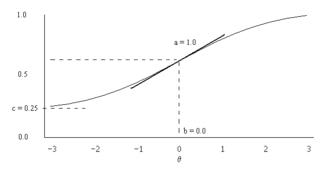
\includegraphics[width=\linewidth]{3PL_IRF.png}
\end{figure}
由上图可以看出$\theta=-3$时被试者仍有概率c答对,对4选1的multiple choice,c=$\frac{1}{4}$,b是$p(\theta)=\frac{c+1}{2}$的点,即最大值1和最小值c的平均值的点,同时也是LRF曲线最陡的点,可以衡量difficulty.a和p'(b)成正比,a越大曲线两级分化越严重,即ability $\theta$小于某一个阈值答对的正确率为c,大于此阈值答对的正确率为1.
此外LRF曲线还可以从标准正态分布的cdf建模。
三个参数的IRF虽然精确,但实际中估计参数比较繁琐,一般常用的是1个参数(b)的Rasch Model,其可以简化表述为第k个person在第i个item上答对的概率为
\begin{equation}\label{eq:Rasch}
P(X_{ki}=1)=\frac{exp(\beta_k-\delta_i)}{1+exp(\beta_k-\delta_i)}
\end{equation}
上式中$\beta_k$表示ability,$\delta_i$表示difficulty.
在获得person $\times$ item的二维表格数据后,要先根据数据估计Rasch Model 的参数$\vec{\delta}=(\delta_1,..\delta_I)$,常用的方法有极大似然法,CML,EM等,关于这三种方法在Rasch Model参数估计的具体讨论,见\ref{A1}。
\subsection{\textbf{\fontsize{12pt}{\baselineskip}{具体实施步骤}}}
下面的列表给出了我们基于Rasch Model关于CAT(computer adapated testing)背单词的实施方案:
\begin{enumerate}
\item{根据课本内容统计词频,归一化后作为每个单词难度的近似替代量}
\item{每一个用户初始化背单词能力为0,每一次背单词后保留其该次背单词能力的估计值,在下一次背单词时采用之前能力值的加权平均值,对于该平均值-单词难度>3的单词则不予考虑,在其他单词中按单词难度进行重要度抽样,样本数量为N个,作为该次背单词的测试集。每次用户的有效测试(没有中途退出和缺失值)保存到服务器的数据库用来更新单词难度。}
\item{定期更新单词难度之前集齐一定数量的测试结果,应考虑到用户的能力变化曲线,有选择地剔除某一部分数据再用CML全局计算单词难度,将计算值与原有的频率值做平均。}
\end{enumerate}
\subsection{\textbf{\fontsize{12pt}{\baselineskip}{单词抽样方法}}}
考虑到总单词数在几百左右,如果分的bins太多,每个bins内单词过少,因为难词多而被抽样的概率低,则大量的难词无法被抽到;简单词少而被抽样的概率高,则简单词几乎必然被抽到。因此在实际操作中,我们把单词分为easy,middle和difficult三类。分类的标准是假设单词难度归一化后是近似指数分布的随机变量X(我们先把单词按从易到难排序,同时用随机模拟的方法生成同样长度的指数分布的随机数,将该随机数序列从小到大排序后作为给定单词总体归一化后的难度),$P(X<1)\approx 64\%,P(X>1 \wedge X<2) \approx 23\%,P(X>2) \approx 13\%$,基于此,我们设定简单词的采样率为
$\frac{10}{13}$,中等词的采样率为$\frac{5}{23}$,难词的采样率为$\frac{3}{64}$,则可以算出三类词在样本中的比率为$10:5:3$,对于给定的单词总体,先将其分成三类;对于给定的样本数N,计算出在简单词类中要无放回的抽取$\frac{10}{18}$,中等词类中抽取$\frac{5}{18}$,难词类中抽取$\frac{3}{18}$.下图是从1000个单词中按上述方法抽取100个单词的模拟结果:
\begin{figure}[!ht]
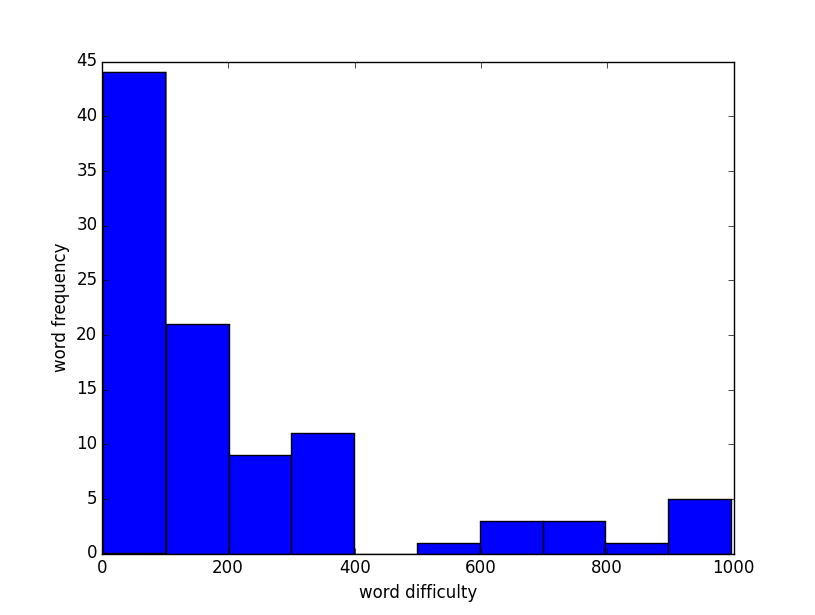
\includegraphics[width=\linewidth]{sampling.png}
\end{figure}

上图中纵轴表示每个bins的大小,横轴是将1000个单词按难度排序,最难的序号为1000,最易的为1。由上图可以看出,
该方法抽到的大部分样本集中在难度排名前20\%的单词,占到样本的60\%以上。
由上面的描述可知,该方法不依赖于单词的绝对难度差异而是根据排名进行的抽样,对于规模为几百的总体,效果较好。
该方法的局限性在于由于每类抽样比固定,对于给定的总体(len=N),样本数量要受到限制,一个比较保守的上限是$\frac{117N}{1000}$,根据概率论\ref{A2}的知识可以计算出当N=200时临界安全概率为99.8\%,即当抽样数恰好等于上界时无放回抽样不会报错的概率为99.8\%,这对于一般的情形
(N$\geq 200$)可认为不安全是小概率事件。
\subsection{\textbf{\fontsize{12pt}{\baselineskip}{Score算法}}}
\subsubsection{算法描述}
Rasche Model算出的ability在测试题目给定的情况下和总分具有非线性的一一对应关系,通过极大似然的方法可以推导出person的ability代数方程
\ref{A3},用牛顿法求解方程即得到ability参数。

实际实现时发现牛顿算法在分数接近满分和接近零分时误差较大,改用优化的方法求$\beta$在[-3,3]区间的极大值则无此问题,下图是利用仿真
数据得到的分数-能力曲线:
\begin{figure}[!ht]
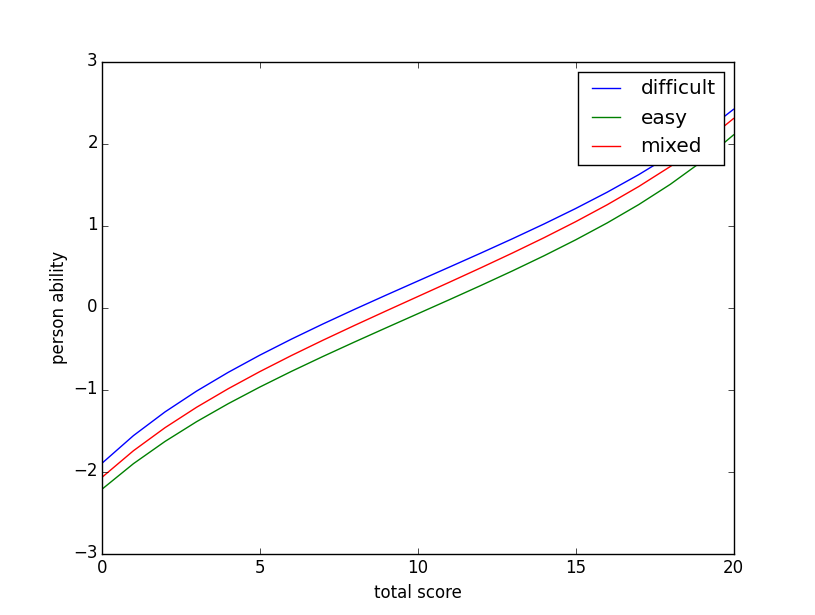
\includegraphics[width=\linewidth]{scoring.png}
\end{figure}

上图中三组数据分别是20个难题,20个容易题,和10个难题和10个容易题的混合组,
由上图可看出每一条曲线有如下特点:
\begin{enumerate}
\item{能力和分数的关系在高分和低分段斜率比较大,非线性性比较明显,而在中部接近线性。}
\item{平均水平能力为0对应答出来一半的题目,曲线具有对称性。}
\end{enumerate}•
比较不同的曲线也符合直观,答出同样数量的题,对于难题组能力高,混合组能力次之,最末为简单题组。
通过用Ability而不是score来衡量从而消除了某一次Test题目的影响而在一个统一的scale上比较。

\subsubsection{精度分析}
对于单次测试而言,可以用总的Fisher信息量$I(\beta)$衡量精度,一般而言,对于某一个估计的值$\hat{\beta}$,$I(\hat{\beta})$越大则表明
估计统计量的方差越小,能力估计的精度越高。\ref{A4}
基于MLE的方法一般都是有偏的,即估计统计量$\hat{\beta}$的均值不等于$\beta$,由于引入了先验的分布,这种偏差在两级状态会非常明显\ref{A5},
下图是比较两组题目bias的结果:
\begin{figure}[!ht]
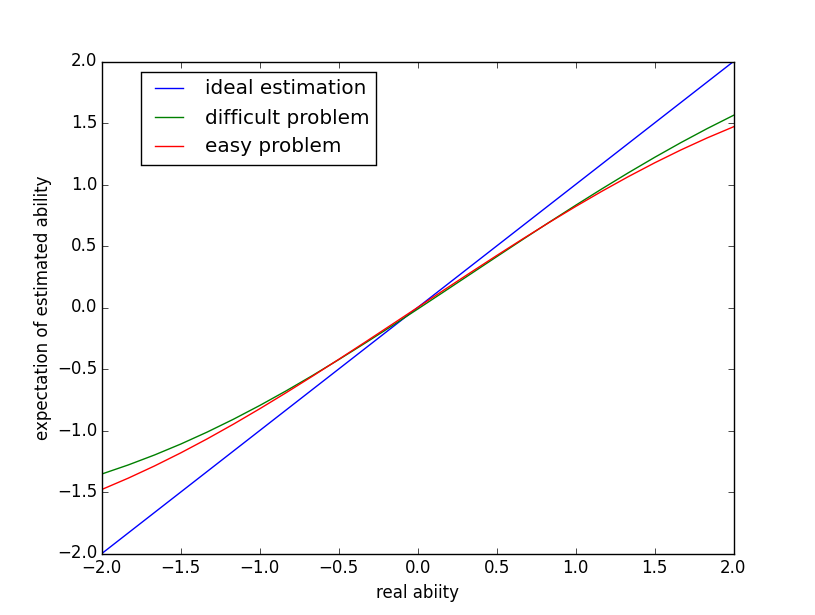
\includegraphics[width=\linewidth]{bias.png}
\end{figure}

如果person的能力接近平均水平(ability $\approx$ 0),则几乎没有bias,但两级的bias会比较大。由于采用了先验的正态总体假设,对于高分,会低估person的能力而对于低分则会高估person的能力。如果题目较难,高分段的bias减小而低分段的bias增大。
\appendix
\section{First Appendix}\label{A1}
\subsection{JML}
首先讨论JML(joint maximum likelihood)的方法,observed data matrix联合概率似然函数为
\begin{equation}
\begin{split}
\log(\Lambda)=\sum_{k=1}^N \beta_k r_k -\sum_{i=1}^I \delta_i s_i+ \\
\sum_{k=1}^N \sum_{i=1}^I \log(1+exp(\beta_k-\delta_i))
\end{split}
\end{equation}
其中$r_k=\displaystyle\sum_{i=1}^I x_{ki}$,表示第k个person的总分,
$s_i=\displaystyle\sum_{k=1}^N x_{ki}$,表示第i个item的总分。
对对数似然函数关于$\delta_i$和$\beta_k$求偏导,得到含$\beta_k$和
$\delta_i$的非线性方程组为
\begin{eqnarray}\label{eq:JML}
s_i=\sum_{k=1}^N p_{ki},i=1,..I\\
r_k=\sum_{i1}^I p_{ki},k=1,..N
\end{eqnarray}•
上式中$p_{ki}$即为(\ref{eq:Rasch})
\subsection{CML}
对实际应用来说,一般N很大,直接求解(\ref{eq:JML})计算量太大。
故一般先求只含item的边缘概率分布,在item的参数$\delta_i$求出的情况下,由于各个person之间相互独立,只需分别对只含一维参数$\beta_k$的函数求极大值点即可。
对第k个person,其各item得分的joint distribution为
\begin{equation}
\begin{split}
P(\vec{x_k}|\beta_k,\vec{\delta})=\prod_{i=1}^I \frac{exp(x_{ki}(\beta_k-\delta_i))}{1+exp(\beta_k-\delta_i)}\\
=\frac{exp(r_k\beta_k)exp(-\sum_{i=1}^I x_{ki}\delta_i)}{\prod_{i=1}^I (1+exp(\beta_k-\delta_i))}
\end{split}
\end{equation}
由$\vec{x_k}$的联合分布可以求出$r_k$的分布为
\begin{equation}
\begin{split}
P(r_k|\beta_k,\vec{\delta})=\sum_{||\vec{y}||_1=r_k}P(\vec{y}|\beta_k,\vec{\delta})\\
=\frac{exp(r_k\beta_k)\displaystyle\sum_{||\vec{y}||_1=r_k}exp(-\sum_{i=1}^I y_{i}\delta_i)}{\prod_{i=1}^I (1+exp(\beta_k-\delta_i))}
\end{split}
\end{equation}
定义$\gamma_{r|\vec{\delta}}=\displaystyle\sum_{||\vec{y}||_1=r}exp(-\sum_{i=1}^I y_{i}\delta_i)$,为elementary symmetric function,则条件似然函数$P(x_k|r_k,\vec{\delta})$为
\begin{equation}
\begin{split}
P(x_k|r_k,\vec{\delta})=\frac{P(x_k|\beta_k,\vec{\delta})}{P(r_k|\beta_k,\vec{\delta})}\\
=\frac{exp(-x_{ki}\delta_i)}{\gamma_{r_k|\vec{\delta}}}
\end{split}
\end{equation}
上式不含$\beta_k$,说明$r_k$是参数$\beta_k$的充分统计量。
由于各person得分相互独立,只需把N个对数似然函数相加即可。
\begin{equation}
\log(\Lambda(\vec{x}|\vec{r},\vec{\delta}))=\sum_{k=1}^N \frac{exp(-x_{ki}\delta_i)}{\gamma_{r_k|\vec{\delta}}}
\end{equation}
\section{Second Appendix}
\subsection{安全概率}\label{A2}
问题可转化为$P(X>2)=0.136,Y_i i.i.d \sim Bernoulli(p=0.136)$,求$P(\displaystyle\sum_{i=1}^N Y_i >K)$
当N较大时,可以用中心极限定理近似计算:
\begin{equation}
P(\frac{\sum_{i=1}^N Y_i-Np}{\sqrt{Np(1-p)}}>\frac{10K/18-Np}{\sqrt{Np(1-p)}})
\end{equation}
上式左边为标准正态分布的随机变量,由上式右边可以看出抽样率K/N必须小于23.4\% (这是该抽样方法最大允许的通过率),否则随着N的增大概率趋近于0.
在实际操作中取$K=\frac{117N}{1000}$满足这个约束,代入N=100可算出概率为98\%,而且N越大安全概率越大。
\subsection{能力参数$\beta$满足的方程}\label{A3}
用$\beta$表示某人的能力,$\beta$的先验分布记成
$p(\beta)$,一般是正态分布,表示在没有考试成绩的时候对其能力的估计,设此人参加了有$i=1,2,..I$个item组成的测试,得分为$x_i$,
每道题的难度为$\delta_i$,由贝叶斯公式,对其成绩的后验估计为:
\begin{equation}
p(\beta|\vec{x})=\frac{p(\beta)p(\vec{x}|\beta)}{p(\vec{x})}\propto p(\beta)p(\vec{x}|\beta)
\end{equation}
$\beta$最有可能的取值为:
\begin{equation}\label{eq:map}
\argmax_{\beta} p(\beta)p(\vec{x}|\beta)
\end{equation}
其中$p(\vec{x}|\beta)$由Rasch Model给出:
\begin{equation}
p(\vec{x}|\beta)=\prod_{i=1}^I \frac{exp(x_i(\beta-\delta_i))}{1+exp(\beta-\delta_i)}
\end{equation}
对含先验分布的对数似然函数\\*
$\log(p(\vec{x}|\beta))$关于$\beta$求导得:
\begin{equation}\label{eq:score}
\frac{p'(\beta)}{p(\beta)}+\sum_{i=1}^I x_i =\sum_{i=1}^I \frac{exp(\beta-\delta_i)}{1+exp(\beta-\delta_i)}
\end{equation}
上面方程的解$\beta$对各项得分的依赖仅仅通过总分$\sum_{i=1}^I x_i$的形式,因此总分是参数$\beta$的充分统计量。由于Rasch  dichotomous Model对person的能力只有一个维度的假定,在items一定的情况下,相同能力与相同总分一一对应。
如果不加先验分布,在全对和全错两种极端情况下方程(\ref{eq:score})无解,因此适当的先验分布是必要的,有用户ability数据的情况下可以拟合正态分布的参数,在缺少用户数据的初始化阶段可以用标准正态分布代替,此时上式第一项化为$-\beta$。
\subsection{Rasch模型Fisher信息量}\label{A4}
$I(\beta)$的计算公式为:
\begin{equation}
I(\beta)=-E(\frac{\partial^2 \log p(\vec{x}|\beta)}{\partial \beta^2})
\end{equation}
对于Rasch Model,代入似然函数表达式,取先验分布为正态分布,则有
\begin{equation}
I(\beta)=1+\sum_{i=1}^I \frac{exp(\beta-\delta_i)}{(1+exp(\beta-\delta_i))^2}
\end{equation}
上式中第一项是先验分布的信息量,后面分别是每一个item的信息量(item infromation function),它们彼此独立因而可以相加。上式的和也被称为
Test Information Function(TIF).
对于每一个item,其IIF有下图所示的形式:
\begin{figure}[!ht]
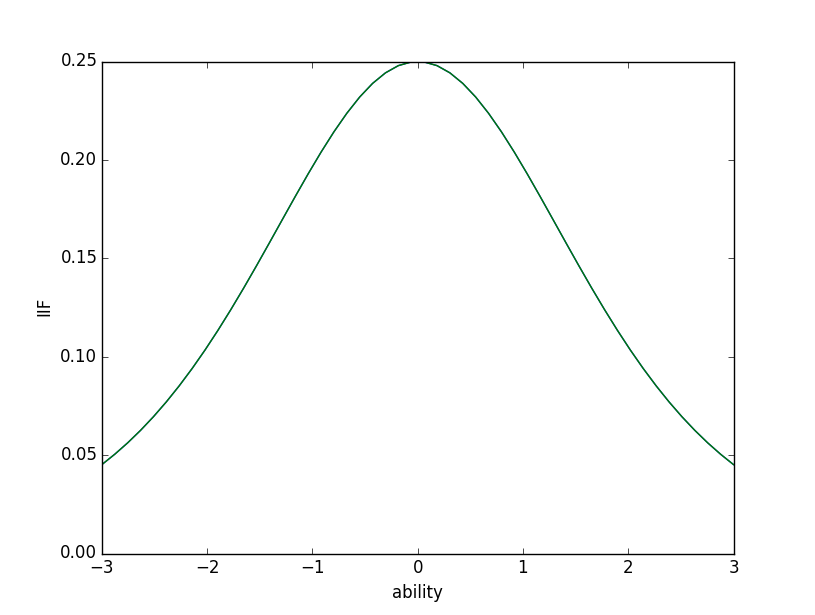
\includegraphics[width=\linewidth]{IIF.png}
\end{figure}

上图是假定item difficulty为0,当$\beta-\delta_i>3$时(题目过难或过易),IIF已经小于0.05,在这种情况下能力估计的误差为比较大。
由于先验分布对TIF的贡献是常数,可以在一定程度上减轻能力的极端情况造成的信息量过少的问题。
下图是20道题的TIF结果:
\begin{figure}[!ht]
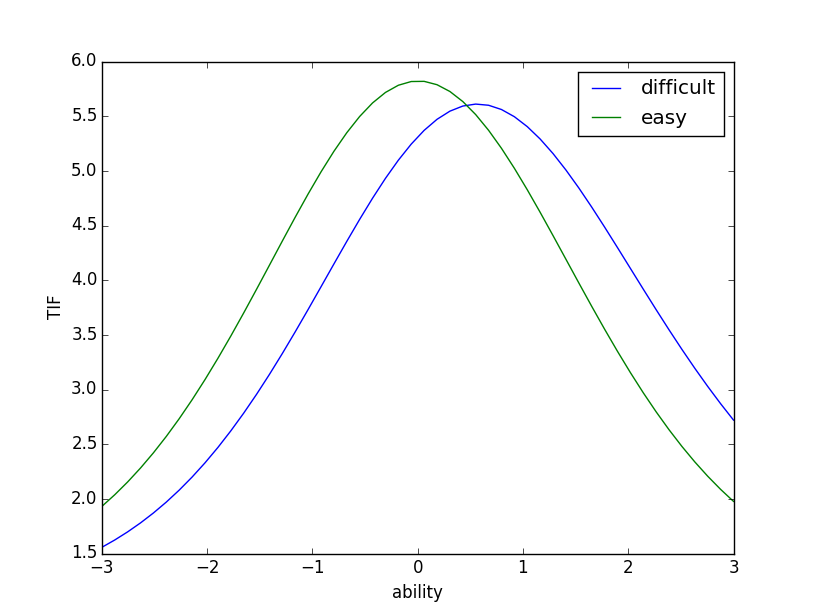
\includegraphics[width=\linewidth]{TIF.png}
\end{figure}

由上图可看出,对于难题组,全对的信息量要比简单题大,而全错的信息量比简单题小,这符合一般经验。
\subsection{Rasch模型Fisher信息量}\label{A5}
计算bias需要计算给定真实能力后计算关于估计量的期望值,在对模型没有任何了解的情况下可以采用Monte Carlo模拟,但对于
Rasch Model由(\ref{eq:score})式得$r_I=\displaystyle\sum_{i=1}^I x_i$是$\beta$的充分统计量,于是首先计算总分$r_I$的分布,
再由
\begin{equation}
E(\hat{\beta}(r_I))=\sum_{i=1}^I \hat{\beta}(i)P(r_I=i)
\end{equation}
计算出期望值。在上式中$\hat{\beta}(i)$可以通过对\ref{eq:map}求解极大值得到,而$r_I$的分布可以类比组合数的计算方法递推得到。
记$A_n^k=\displaystyle\sum_{k=1}^n x_k$,则有如下递推公式:
\begin{equation}
A_n^k=P(x_n=1)A_{n-1}^{k-1}+P(x_n=0)A_{n-1}^k
\end{equation}
上式中$P(x_n=1)$为第n道题的答对概率。
该方法计算规模为$O(n^3)$,其中n为item 数量,相比Monte Carlo模拟需要大量重复才能得到比较精确的结果在n不大时效率比较高。
%信息量和能力估计的标准差$\sigma_{\hat{\beta}}$之间的关系很难给出理论表达式,
%但可以用$\frac{1}{\sqrt{I(\hat{\beta})}}$近似作为标准差的下界。
\begin{thebibliography}{}
\bibitem{Bib1}双语学习型词典设计特征研究 外研社2013年出版

\bibitem{Bib2} 计算词典学 上海辞书出版社2011年版

\bibitem{Bib3} \url{https://github.com/Leidenschaft/Deutsch-Lernen}
\bibitem{Bib4} How Many Words Do We Know? Practical Estimates Of
Vocabulary Size Depedenent on Word Definition, the Degree of Language Input and the Participant's Age		frontiers in Psychology
\end{thebibliography}
\end{document}